\documentclass{article}

\usepackage{pgfplots}
\usepackage[margin=1in]{geometry}

\title{Assignment 2: MPI}
\author{Elijah Kin}
\date{October 10, 2024}

\begin{document}
  \maketitle

  \subsection*{Data Distribution}
  We first have process 0 read in the entire input file to a \texttt{global\_life} 1D array. We then scatter this array across all processes, each receiving a chunk of the board into their own \texttt{life} array (also now 1D). Each process also has its own local \texttt{previous\_life} array.

  Then in each generation, each process sends the top and bottom rows of its \texttt{life} array to the ghost rows in the \texttt{previous\_life} arrays of its neighboring processes. Finally after performing all iterations, we gather from all processes back into the \texttt{global\_life} array on process 0, before writing to an output file.

  \subsection*{Performance Results}
  Running the program on the 512x512 board for 500 iterations as a benchmark, we measure the following execution times on Zaratan.
  \begin{center}
    \begin{tabular}{ |c|c|c|c|c|c|c| }
      \hline
      Processes & 4 & 8 & 16 & 32 & 64 & 128 \\
      \hline
      Min (s) & 0.064236 & 0.03386 & 0.029902 & 0.042488 & 0.092184 & 0.14385 \\
      \hline
      Avg (s) & 0.0649503 & 0.0374385 & 0.0425478 & 0.0803294 & 0.169988 & 0.273515 \\
      \hline
      Max (s) & 0.066074 & 0.043119 & 0.051057 & 0.090568 & 0.196102 & 0.306212 \\
      \hline
     \end{tabular}
  \end{center}
  We also display the same data in a line plot below.
  \begin{center}
    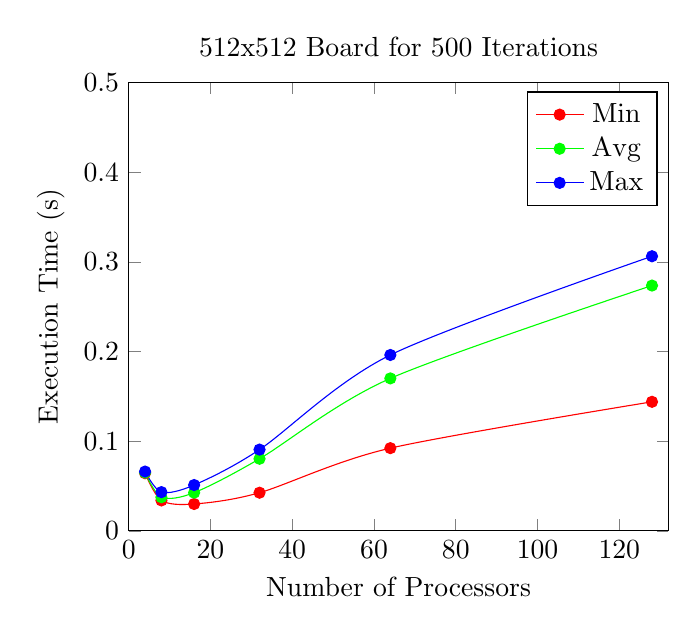
\begin{tikzpicture}
      \begin{axis}[
          title=512x512 Board for 500 Iterations,
          xlabel=Number of Processors,
          ylabel=Execution Time (s),
          xmin=0, xmax=132,
          ymin=0, ymax=0.5]
      \addplot[smooth, mark=*, red] plot coordinates {
          (4, 0.064236)
          (8, 0.03386)
          (16, 0.029902)
          (32, 0.042488)
          (64, 0.092184)
          (128, 0.14385)
      };
      \addlegendentry{Min}

      \addplot[smooth, mark=*, green] plot coordinates {
          (4, 0.0649503)
          (8, 0.0374385)
          (16, 0.0425478)
          (32, 0.0803294)
          (64, 0.169988)
          (128, 0.273515)
      };
      \addlegendentry{Avg}

      \addplot[smooth, mark=*, blue] plot coordinates {
          (4, 0.066074)
          (8, 0.043119)
          (16, 0.051057)
          (32, 0.090568)
          (64, 0.196102)
          (128, 0.306212)
      };
      \addlegendentry{Max}
      \end{axis}
    \end{tikzpicture}
  \end{center}
  Observe that the plots for Avg and Max are quite close to each other, suggesting an approximately equal work distribution. Further, we expect that in the limit, Min is approximately half of Avg, since the first and last processes only communicate half as much as the others.
\end{document}
